\chapter{Wyniki eksperymentów}
\label{c5}

\section{Wstęp}
\label{c51}
W poniższym rozdziale opisano przebieg przeprowadzonych eksperymentów oraz przedstawiono uzyskane wyniki wraz z ich interpretacją. Algorytmy testowane były na tych samych zbiorach danych. Tworzenie tych zbiorów odbywało się z wykorzystaniem generatora przyjmującego jako parametry liczbę transakcji (np. 10 tys., 100 tys.), średnią liczbę elementów w transakcji (np. 6), liczbę wzorców do odkrycia (np. 500), średni rozmiar wzorców częstych do odkrycia (np. 3), liczbę różnych elementów występujących w transakcjach (np. 1000, 10000) oraz nazwę pliku wyjściowego. Wygenerowany plik jest importowany do bazy danych, do której odwołuje się aplikacja podczas wykonywania algorytmów. Dane w bazie składowane są w jednej tabeli w postaci par \((id transakcji, id elementu)\). Dlatego też po odczycie tej tabeli składane są transakcje wykorzystywane w dalszym przetwarzaniu. Zbiór zapytań \(DMQ\) generowany był przed rozpoczęciem przetwarzania. Liczba transakcji obejmująca każde zapytanie \(dmq_i\) wynosi \(|T|/|DMQ|\), gdzie \(|T|\) - liczba wszystkich transakcji, \(|DMQ|\) - liczba wszystkich zapytań eksploracyjnych. 

\section{Opis infrastruktury}
\label{c52}
Algorytmy napisane zostały w języku Java, z wykorzystaniem narzędzia Maven oraz środowiska programistycznego Eclipse. Dane testowe generowane były za pomocą generatora GEN (\cite{AgrawalGEN}), a następnie wczytywane do bazy PostgreSQL, z której korzystała aplikacja. Testy przeprowadzone zostały na komputerze HP Envy 14 Notebook PC, z procesorem Intel Core i5-2410M 2x2.30GHz oraz 8GB pamięci RAM, pracującym pod kontrola systemu operacyjnego Microsoft Windows 7. 

\section{Wyniki}
\label{c53}
Poniżej zaprezentowano wyniki eksperymentów. Wszystkie uwzględnione czasy są średnią 4 dokonanych pomiarów dla dokładnie tych samych parametrów. Badania przeprowadzono dla dwóch zapytań eksploracyjnych z różnym poziomem nakładania się danych. Oba zapytania wykorzystywały ten sam próg wsparcia, mimo że nie jest to wymaganiem algorytmu. Jest to podyktowane chęcią możliwości lepszego zaobserwowania różnic w działaniu algorytmów niezależnie od wykorzystywanych progów dla poszczególnych zapytań. 

Zbiór danych 1.\newline
Parametry generatora dla drugiego zbioru danych przedstawia tabela \ref{table:firstDataSetParams}.
\begin{table}[h]
\begin{center}
	\begin{tabular}{| l | c |}
		\hline
		liczba transakcji & 100000 \\ \hline
		średnia liczba elementów w transakcji & 8 \\ \hline
		liczba różnych elementów & 1000 \\ \hline
		liczba wzorców (zbiorów częstych) & 1500 \\ \hline
		średnia liczba elementów we wzorcu & 4 \\ 
		\hline
	\end{tabular}
\end{center}
\caption{Parametry generatora dla pierwszego testowego zbioru transakcji.}
\label{table:firstDataSetParams}
\end{table}

\begin{figure}[h]
	\centering
	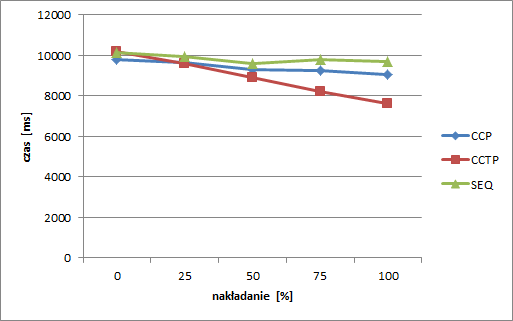
\includegraphics[width=0.8\linewidth]{figures/chart_100_2}
	\caption{Wykres dla pierwszego zbioru danych dla dwóch zapytań \(dmq\) z różnym stopnieniem nakładania się i \(minsup = 2\)}
	\label{fig:chart_100_2}
\end{figure}

\begin{figure}[h]
	\centering
	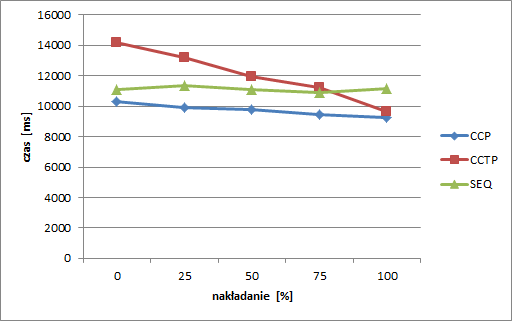
\includegraphics[width=0.8\linewidth]{figures/chart_100_1}
	\caption{Wykres dla pierwszego zbioru danych dla dwóch zapytań \(dmq\) z różnym stopnieniem nakładania się i \(minsup = 1\)}
	\label{fig:chart_100_1}
\end{figure}


Zbiór danych 2.\newline
Parametry generatora dla drugiego zbioru danych przedstawia tabela \ref{table:secondDataSetParams}.
\begin{table}[h]
	\begin{center}
		\begin{tabular}{| l | c |}
			\hline
			liczba transakcji & 50000 \\ \hline
			średnia liczba elementów w transakcji & 8 \\ \hline
			liczba różnych elementów & 1000 \\ \hline
			liczba wzorców (zbiorów częstych) & 1000 \\ \hline
			średnia liczba elementów we wzorcu & 4 \\ 
			\hline
		\end{tabular}
	\end{center}
	\caption{Parametry generatora dla drugiego testowego zbioru transakcji.}
	\label{table:secondDataSetParams}
\end{table}

\begin{figure}[h]
	\centering
	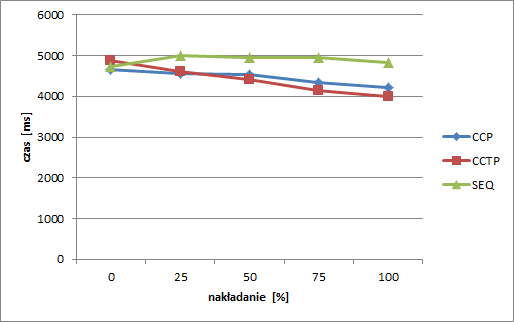
\includegraphics[width=0.8\linewidth]{figures/chart_50_2}
	\caption{Wykres dla drugiego zbioru danych dla dwóch zapytań \(dmq\) z różnym stopnieniem nakładania się i \(minsup = 2\)}
	\label{fig:chart_50_2}
\end{figure}

\begin{figure}[h]
	\centering
	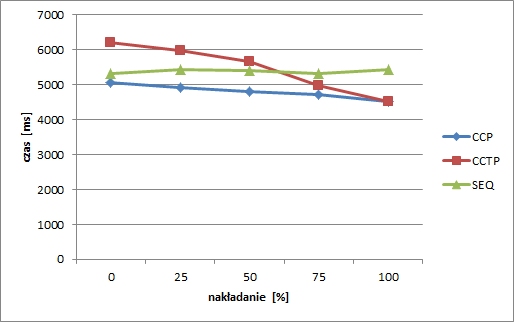
\includegraphics[width=0.8\linewidth]{figures/chart_50_1}
	\caption{Wykres dla drugiego zbioru danych dla dwóch zapytań \(dmq\) z różnym stopnieniem nakładania się i \(minsup = 1\)}
	\label{fig:chart_50_1}
\end{figure}


\section{Dalsze prace}
\label{c54}
Adaptacje algorytmu Apriori oraz algorytmy przetwarzające zbiory zapytań eksploracyjnych nadal mogą być ulepszane i optymalizowane. Jednym z możliwych rozwiązań jest próba wykorzystania Common Counting w taki sposób, że na podstawie zbioru elementarnych predykatów selekcji danych dla zbioru zapytań eksploracyjnych \(S\) generowane są rozłączne zapytania \(dmq_i\), dla których algorytm wykonywany jest w ten sam sposób jaki opisano w \ref{c43}. Ostatnim krokiem byłaby wówczas integracja znalezionych zbiorów częstych w celu uzyskania odpowiedzi na oryginalne zapytania ze zbioru \(DMQ\). Takie podejście zmniejszyłoby rozmiary drzew przechowujących kandydatów podczas przetwarzania. Należałoby sprawdzić czy zysk ten jest większy niż koszt operacji generowania zbioru rozłącznych zapytań \(DMQ\). 

Innym zagadnieniem jest problem optymalizacji generowania kandydatów dla CCTP. Sortowanie wartości podczas dodawania jest czasochłonne, mimo że porównywane są jedynie dwie wartości zbioru elementów, a nie cała lista wartości. Mimo prób zastosowania innych struktur (m.in. zbioru czy też drzew haszowych) podczas tej operacji nie udało się uzyskać lepszego wyniku niż dla ostatecznie zastosowanego rozwiązania. 